\documentclass{article}
\usepackage[romanian]{babel}
\usepackage{graphicx}
\title{RECAPITULARE}
\author{anul IAC}
\sloppy
\begin{document}
\maketitle
\section{Cadre și comenzi în modul matematic}\label{mat}
Secțiunea \ref{mat} are contorul \verb+section+ cu valoarea \thesection.
\paragraph{O matrice}
Cadrul \verb+array+ se deschide doar în modul matematic.
$$
A=\left[
\begin{array}{rr}
0&1\\
-1&\frac{1}{2}
\end{array}
\right]
$$
\paragraph{O ecuație}
Cadrul \verb+equation+  deschide modul matematic și e numerotat cu contorul \verb+equation+.
\begin{equation}
f(x)=f(x_{0})+...
\end{equation}
\paragraph{Mai multe ecuații}
Cadrul \verb+eqnarray+ deschide modul matematic și are o structură \verb+array+ cu 3 coloane.
\begin{eqnarray}
\sin \frac{\pi}{4}&=&\frac{\sqrt{2}}{2}\\
%\nonumber
\cos 0&=&1
\end{eqnarray}
\section{Cadre și comenzi în modul text}
\paragraph{Un tabel}
Cadrul \verb+table+ e numerotat automat iar corpul tabelului este creat cu \verb+tabular+.
\begin{table}[htpb]
\begin{tabular}{ll}
\multicolumn{2}{c}{Un text extins}\\\hline
1&o celulă\\\hline
\end{tabular}
\caption{O legendă.}\label{tab:tab}
\end{table}
Pentru centrarea tabelului folosim \verb+\centering+. Aici nu e centrat.
\paragraph{Alinierea paragrafelor}
\begin{center}
Text centrat
\end{center}
\begin{flushright}
Text la dreapta
\end{flushright}
\begin{flushleft}
Text la stânga.
\end{flushleft}
\paragraph{Liste}
O listă nenumerotată, cu cadrul \verb+itemize+, cu sub-listă nenumerotată și numerotată, cu cadrul \verb+enumerate+.
\begin{itemize}
\item Un element principal
\begin{itemize}
\item Un element secundar
\end{itemize}
\item Alt element principal
\begin{enumerate}
\item Alt element secundar \label{alt_secund}
\begin{enumerate}
\item Un element secundar al elementului secundar \ref{alt_secund} \label{alt_secund_secund}
\end{enumerate}
\end{enumerate}
\end{itemize}
Contorul \ref{alt_secund_secund} al sub-elementului din \ref{alt_secund}. \\
Listele etichetate se scriu cu cadrul \verb+description+.
\paragraph{Inserarea de grafică}
Cadrul \verb+figure+ e numerotat cu contorul cu același nume, similar cu cadrul \verb+table+.
\begin{figure}[b]
\centering
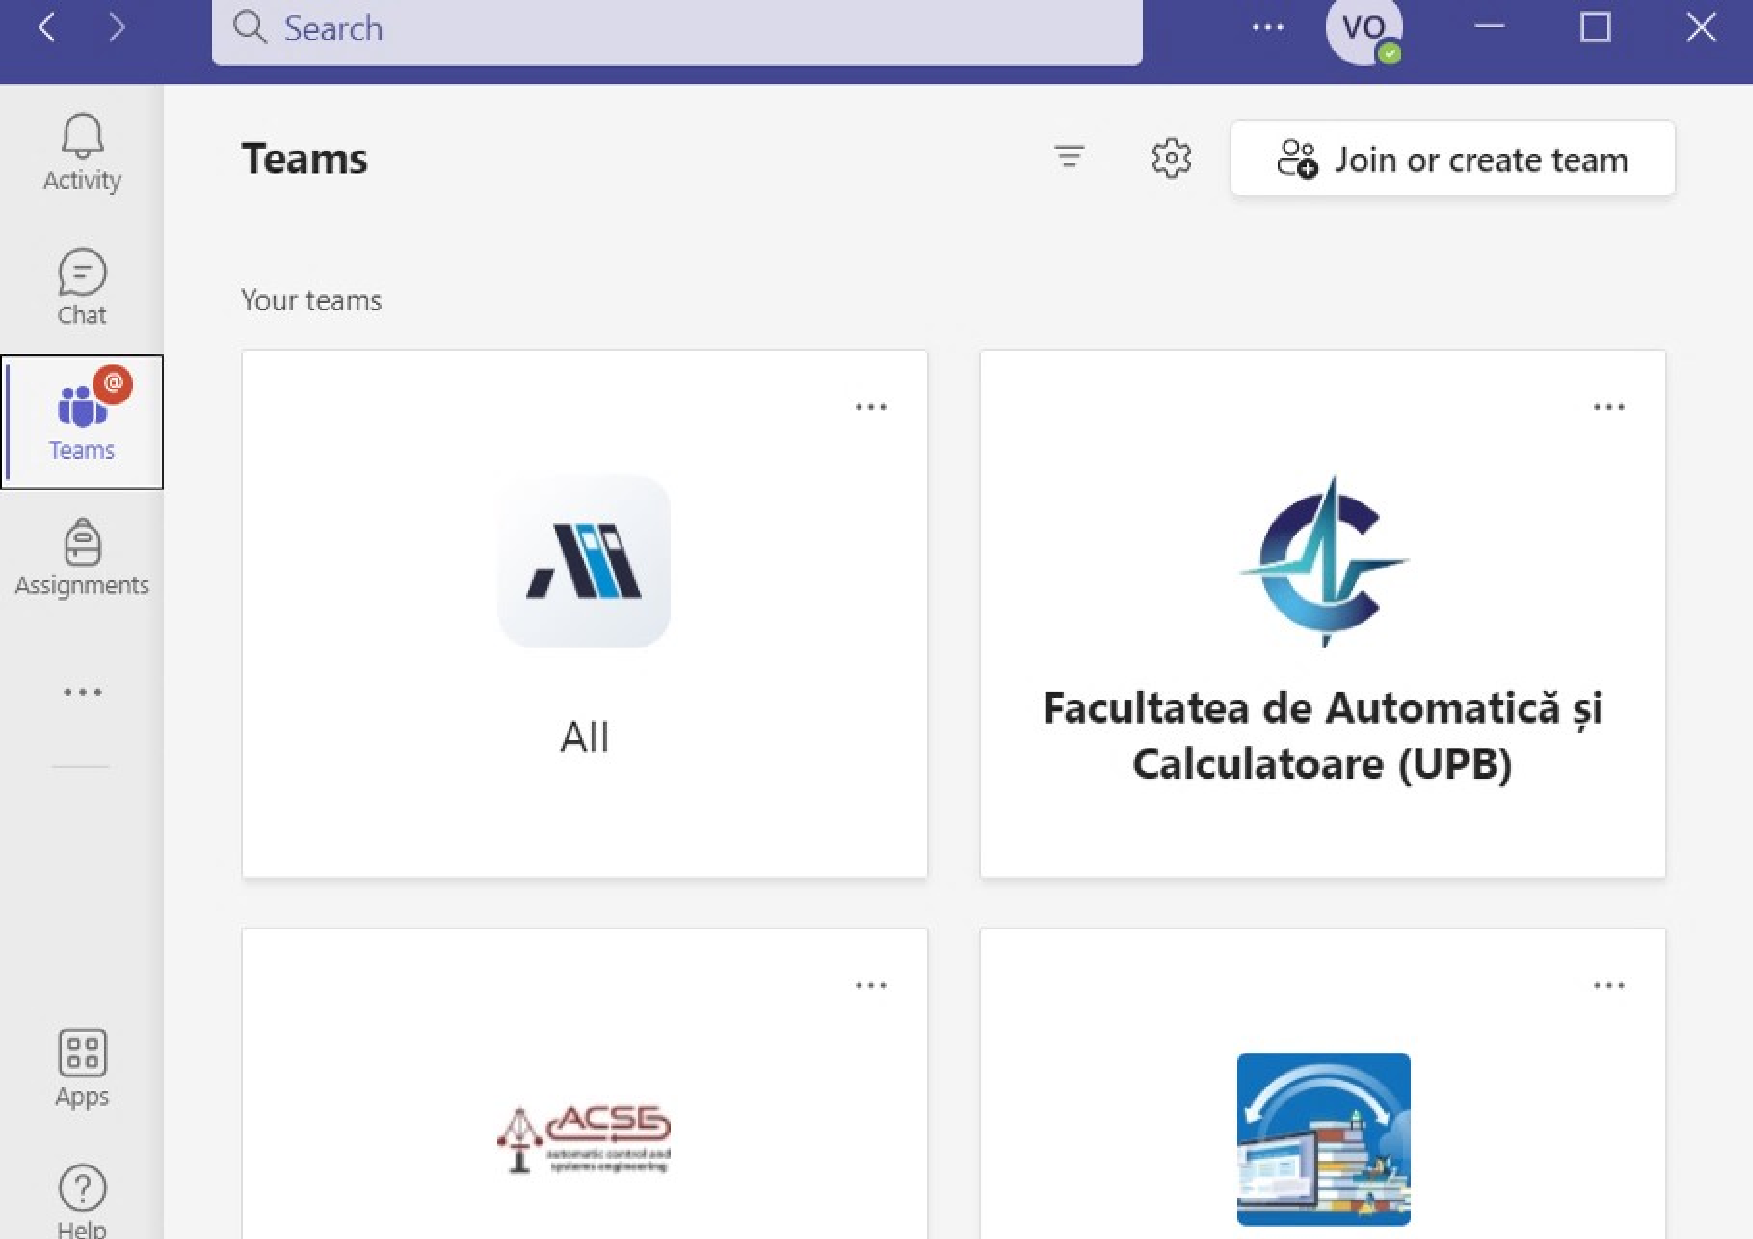
\includegraphics[scale=0.2]{poza.pdf}
\caption{O poză}
\end{figure}
\paragraph{Cum scriem linii de program?}
Folosim cadrul \verb+tabbing+
\begin{tabbing}
var=0\\
fo\= r i=1:n\\
\> var=var+1 % \+
\\
end
\end{tabbing}
\paragraph{Bibliografie creată manual}
Lucrarea \cite{aut} conține un capitol despre funcțiile de variabila complexă. Am creat o bibliografie etichetată.
\begin{thebibliography}{aaaaaaaaaa}
\bibitem[Pop,21]{aut} Ion Pop, Matematici speciale, Ed.ALL, 2021.
\bibitem[Ionescu,20]{ion} Mihai Ionescu, Analiza matematică, Ed. Politehnica Press, 2020.
\end{thebibliography}

\end{document}